\section{Historical: Retained Negative Follow-Ups}
These studies tested possible improvements before the broad comparisons.
None changed the three original 188-parameter checkpoints. Their outcomes
are kept separate because they use different test banks and budgets.

\subsection{A Controller Around OptShrink}
The first hybrid used a learned mixing rule around OptShrink. On 704 fresh
worlds, its seven-SNR average was $-14.129$~dB, compared with
$-14.535$~dB for the stronger OptShrink control. It therefore lost
0.406~dB. Its ten-stage schedule and some ranks did not match the strong
baseline. A clipped gate also had zero local derivative in many high-SNR
cases. These were reasons to repair the comparison, not evidence that
repairing it would produce an improvement.

The corrected pilot used the strong baseline's ranks and noise-dependent
iteration schedule, removed the hard clipping, and trained two
initializations on one shared dataset. Settings were fixed before 704 new
test worlds were generated. The learned gate started at 0.95 where the
baseline used strength one; a near-initial control accounted for this
difference. Table~\ref{tab:hybrid-retained} gives the primary seven-SNR
averages. Four stress cells were reported separately.

\begin{table}[!t]
\caption{Corrected hybrid pilot: lower NMSE is better.}
\label{tab:hybrid-retained}\centering\small
\begin{tabular}{@{}lr@{}}\toprule
Method & NMSE (dB)\\\midrule
Strong OptShrink & $-14.596$\\
Retuned classical mixing & $-14.637$\\
Residual-based classical rule & $-14.633$\\
Stage-only learned mixing & $-14.656$\\
Corrected measurement-conditioned hybrid & $-14.616$\\\bottomrule
\end{tabular}
\end{table}

The corrected hybrid gained only 0.019~dB over the strong starting
baseline, with conditional pointwise 95\% interval
$[0.004,0.033]$~dB. It lost 0.022~dB to retuned classical mixing and
0.040~dB to the simpler stage-only learned rule. Mean same-backend
processing times were about 7.2~ms for the hybrid and 6.2~ms for
OptShrink. The corrected gate had no exact-zero local slopes in the
recorded tests, but this did not make it the better estimator. The
screen failed, and the hybrid was not expanded. Its numerical audit
regenerated 2,720 worlds and checked 198 checkpoint predictions and
11 independent classical predictions.

\subsection{Stopping, Filter Release and a Larger Learned Control}
A separate 704-world pilot included two independent 352-world banks,
each with 32 worlds in seven primary and four stress cells. The first
bank tested observable stopping and releasing the structural filter.
Frozen OptShrink, observed stopping and observed release reached
$-14.530$, $-14.498$ and $-14.449$~dB, respectively. Release lost
0.050~dB to observed stopping and 0.081~dB to frozen OptShrink. Stopping
improved the weak-reference diagnostic, but not the primary average.
It computed all 100 updates before choosing an output; its selected
iteration count was not its total processing cost.

The second bank compared a newly trained compact model with an
independently implemented exact-EM Transformer with 1,585,920 parameters.
Both used 4,096 training cases, 12 epochs, matching masks and order,
one training seed, and held-out likelihood for selection. Selected
NMSEs were $-14.325$~dB for the compact model, $-9.726$~dB for the
Transformer, $-14.289$~dB for OptShrink and $-10.116$~dB for EM100.
The compact--OptShrink gain interval, $[-0.095,0.176]$~dB, included zero.
The Transformer was worse than EM100, so this pilot did not provide a
strong learned comparator. It was not a reproduction of published
URformer and supports no superiority claim over that method. Neither
training budget establishes convergence.

\subsection{An Error-Model Feasibility Check}
A further screen examined whether local sensitivity could predict the
error entering a Hankel filter. It used 24 fixed channel/pilot/reference
worlds, 256 repeated noise draws and eight separate prediction anchors
per world. Noise repetitions were not new channel realizations. The
ordinary-start covariance check passed six of ten primary groups,
below its required eight; the total-error/bias check passed seven.
At SNR $-10$~dB after 100 EM updates, predicted variance was 16.48
times observed variance. With a weak reference it was 5.72 times.
Estimated bias accounted for about 57\% of total error at 20 updates
and 22\% at 100 updates in the weak-reference group.

Two supplementary finite-difference checks exceeded their original
tolerance. Smaller steps and independent automatic differentiation
resolved the numerical discrepancy. Ordinary-start relative Jacobian
errors in the two problematic settings were about 0.0113\% and
0.0023\%, too small to explain the main prediction failure. The
scientific screen remained failed. This study concerned unfiltered,
row-separable EM; it did not validate an error model for interleaved
Hankel reconstruction or establish an optimal shrinker. No new filter
was promoted on the basis of these predictions.

\subsection{What These Checks Leave Open}
An observable likelihood score is not a channel-error guarantee. A
smooth gate is not enough to establish useful adaptation. More network
parameters do not establish a stronger trained baseline. The retained
failures narrow the claim to the tested original compact estimator;
they do not supply evidence for a new hybrid, an uncertainty-aware
filter or a general improvement to OptShrink.

\subsection{Retained Figures From the Earlier Studies}
These plots retain the earlier narrow-population and operating-limit
results. They use the protocols stated in their captions, not the
new broad-study test banks.
\begin{figure*}[!t]
\centering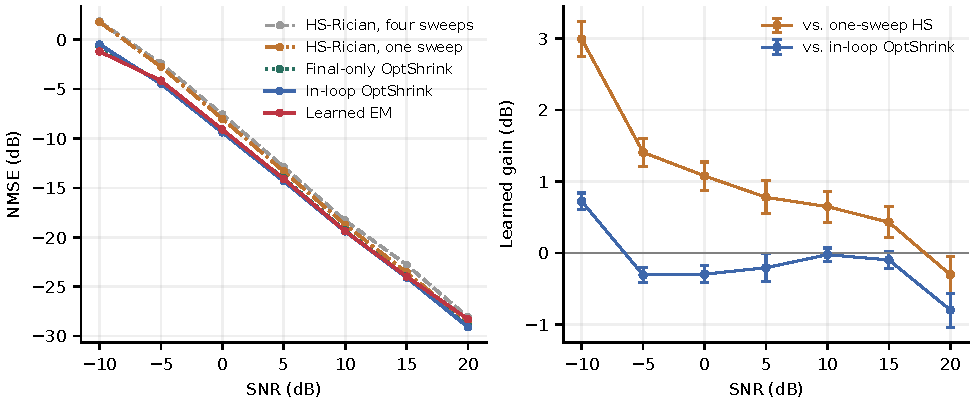
\includegraphics[width=\textwidth]{optshrink.pdf}
\caption{Earlier narrow-population comparison: 128 paired trials per SNR
and frozen learned models. The one-sweep HS-Rician result was added on
the same saved worlds. Right: learned gains over one-sweep HS-Rician
and in-loop OptShrink; positive favors learning. Intervals are pointwise
and condition on the saved models.}
\end{figure*}
\begin{figure*}[!t]
\centering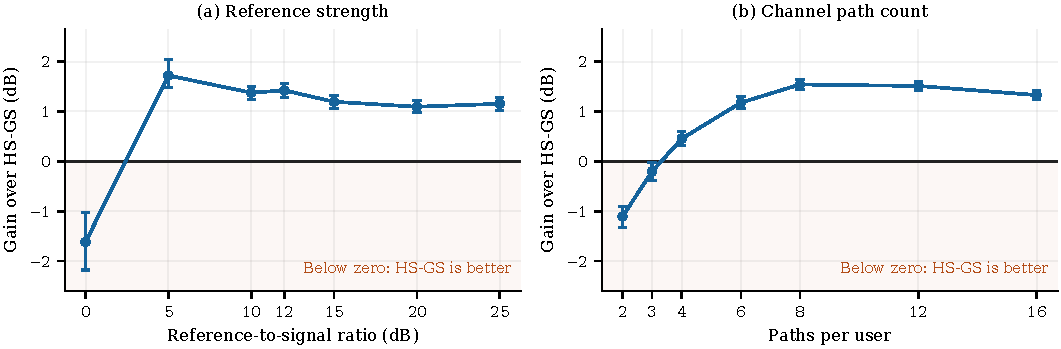
\includegraphics[width=\textwidth]{learned_limits.pdf}
\caption{Limits in the original learned study at SNR 5~dB.
(a) Reference strength for three-to-seven-path channels.
(b) Fixed path counts at RSR 12~dB. Gains compare adaptive EM with
four-sweep HS-amplitude (HS-GS in the plot). Bars are conditional
pointwise paired intervals; tested path counts overlap training.}
\end{figure*}
